%% Informe técnico del Proyecto Final, Electiva en Ingeniería de Software
%% Universidad de San Buenaventura Cali, plantilla elsarticle (preprint, 12pt)
\documentclass[preprint,12pt]{elsarticle}

\usepackage[utf8]{inputenc}
\usepackage[T1]{fontenc}
\usepackage[spanish,es-tabla,es-nodecimaldot]{babel}
\spanishdeactivate{<>}
\usepackage{amssymb}
\usepackage{amsmath}
\usepackage{graphicx}
\usepackage{booktabs}
\usepackage{array}
\usepackage{tikz}
\usetikzlibrary{arrows.meta,positioning}
\usepackage[labelsep=period]{caption}
\usepackage[hidelinks]{hyperref}
\usepackage{url}
\setlength{\emergencystretch}{2em}
\setlength{\textfloatsep}{10pt plus 2pt minus 2pt}
\setlength{\floatsep}{8pt plus 2pt minus 2pt}
\setlength{\intextsep}{8pt plus 2pt minus 2pt}
\renewcommand{\topfraction}{0.92}
\renewcommand{\bottomfraction}{0.8}
\renewcommand{\textfraction}{0.06}
\renewcommand{\floatpagefraction}{0.85}
\setcounter{topnumber}{3}
\setcounter{totalnumber}{5}

\journal{Electiva en Ingeniería de Software}
\abstracttitle{Resumen}
\keywordtitle{Palabras clave}
\usepackage{etoolbox}
\makeatletter
\patchcmd{\ps@pprintTitle}{Preprint submitted to}{Documento presentado a}{}{\PackageWarning{informe}{No se pudo cambiar el pie de página}}
\makeatother

\begin{document}

\begin{frontmatter}

\title{Clasificación de especies de árboles urbanos con aprendizaje profundo sobre nubes de puntos LiDAR aéreas}

\author{Julian David Fuentes Granja}
\affiliation{organization={Facultad de Ingeniería, Universidad de San Buenaventura Cali},
            city={Cali},
            country={Colombia}}

\begin{abstract}
Este trabajo clasifica la especie de árboles urbanos aislados a partir de nubes de puntos LiDAR aéreas con el dataset público UrbanTree3D, que tiene 152 árboles de seis especies validadas en campo. Se compararon PointNet, PointNet++ y DGCNN con un bosque aleatorio sobre descriptores geométricos en cuatro experimentos, que son la partición oficial, el número de puntos por árbol, el uso de la intensidad y los retornos del LiDAR y una validación cruzada estratificada repetida con pruebas estadísticas corregidas. En la partición oficial DGCNN alcanzó un F1 macro de 0.964, pero en validación cruzada bajó a 0.841, lo que muestra que esa partición es optimista. La mejora más clara vino de los atributos del sensor, con los que PointNet llegó a una exactitud de 0.928 y un F1 macro de 0.914 en validación cruzada, frente a 0.853 del mejor bosque aleatorio. Con 152 árboles, las pruebas con corrección de Holm solo confirmaron que PointNet++ sin atributos es inferior a las dos mejores redes con atributos.
\end{abstract}

\begin{keyword}
Nubes de puntos \sep Aprendizaje profundo \sep Arbolado urbano \sep Clasificación de especies \sep LiDAR aéreo
\end{keyword}

\end{frontmatter}

%% =====================================================================
\section{Introducción}
\label{sec:intro}

El inventario de la vegetación urbana sirve para evaluar la salud ambiental, el riesgo de caída de árboles y la planeación de la siembra. Los árboles urbanos sostienen parte de la biodiversidad de las ciudades \cite{jovanovic2025urbantrees}, y para gestionarlos hay que saber dónde está cada uno y de qué especie es. Ese dato se ha levantado con censos manuales en terreno, que son lentos y caros, o con fotografías aéreas 2D, que sufren por las sombras y no capturan el volumen, la forma de la copa ni la altura. El LiDAR aerotransportado resuelve esa limitación porque entrega la geometría tridimensional de la ciudad, y en contextos urbanos sigue siendo más preciso que los productos globales de altura de dosel \cite{dong2025highprecision}.

Este trabajo busca responder si una red neuronal que recibe directamente la nube de puntos de un árbol puede reconocer su especie mejor que un método clásico basado en medidas de la copa, cuando se tiene un dataset pequeño de árboles urbanos escaneados desde un avión. Para responderlo se entrenaron tres redes conocidas para nubes de puntos, PointNet, PointNet++ y DGCNN, y se compararon con un bosque aleatorio que usa descriptores geométricos calculados a mano. Todas las redes se programaron en PyTorch y se entrenaron en Google Colab.

El trabajo hace tres aportes. El primero es una comparación de las cuatro opciones bajo las mismas condiciones en el dataset UrbanTree3D, que hasta ahora solo se había evaluado con una red. El segundo es medir qué tanto cambian los resultados al variar el número de puntos por árbol y al agregar la intensidad y los retornos del láser. El tercero es una evaluación con validación cruzada repetida y pruebas estadísticas, porque con 26 árboles de prueba la partición oficial deja mucho espacio al azar. Además se muestran las curvas de entrenamiento y validación de cada red y ejemplos de lo que predice el modelo frente a la especie real.

El documento sigue este orden. La sección~\ref{sec:problema} define el problema, la sección~\ref{sec:estado-arte} resume el estado del arte, la sección~\ref{sec:metodos} explica el dataset, las redes y los experimentos, la sección~\ref{sec:resultados} presenta los resultados, la sección~\ref{sec:discusion} los discute y la sección~\ref{sec:conclusiones} cierra con las conclusiones y el trabajo futuro.

\section{Descripción del problema}
\label{sec:problema}

La entrada del sistema es una nube de puntos desordenada $P=\{p_1,\dots,p_n\}$, donde cada punto tiene coordenadas $(x_i,y_i,z_i)$ y atributos del sensor como la intensidad $I_i$ y el número de retorno $r_i$.
\begin{equation}
P = \{p_i\}_{i=1}^{n}, \qquad p_i = (x_i, y_i, z_i, I_i, r_i).
\label{eq:pointcloud}
\end{equation}
El problema completo tiene dos etapas, y la primera separa la nube de la escena en $K$ árboles individuales con una función de asignación $s$, donde $k=0$ representa el fondo.
\begin{equation}
s : P \rightarrow \{0, 1, \dots, K\}, \qquad P_k = \{p_i \in P : s(p_i) = k\}.
\label{eq:instancias}
\end{equation}
La segunda asigna una especie a cada árbol aislado con una red neuronal $f_\theta$ de parámetros $\theta$.
\begin{equation}
f_\theta : P_k \rightarrow \{1, \dots, C\}, \qquad C = 6.
\label{eq:clasificacion}
\end{equation}

El dataset usado, UrbanTree3D, ya trae resuelta la primera etapa porque sus autores aislaron cada árbol con DBSCAN y Watershed \cite{hamdani2026hybrid,hamdani2026urbantree3d}, así que este trabajo se concentra en la ecuación~\eqref{eq:clasificacion}. El alcance se ajustó frente a la primera entrega, que planteaba una segmentación por punto, porque UrbanTree3D tiene una etiqueta de especie por árbol y no por punto.

El notebook ejecutado y los resultados del entrenamiento están en el repositorio público \url{https://github.com/JDav19/arbolado-urbantree3d}.

%% =====================================================================
\section{Estado del arte}
\label{sec:estado-arte}

\subsection{Aprendizaje profundo sobre nubes de puntos}

El procesamiento de nubes de puntos pasó de convertir los datos a vóxeles o a proyecciones 2D a trabajar directamente sobre conjuntos desordenados de puntos, una evolución que Guo et al. organizaron en una revisión de clasificación, detección y segmentación \cite{guo2021survey}. PointNet fue la primera red en aplicar un perceptrón compartido a cada punto y juntar el resultado con un máximo simétrico, lo que la hace invariante al orden de los puntos \cite{qi2017pointnet}, aunque no modela vecindarios locales. PointNet++ corrigió esa limitación con una jerarquía de agrupamientos por radio que aplica PointNet de forma recursiva \cite{qi2017pointnetpp}, y DGCNN propone la convolución de aristas EdgeConv sobre un grafo de vecinos que se recalcula en el espacio de características de cada capa \cite{wang2019dgcnn}.

PointNeXt mostró que buena parte de la ventaja de los modelos recientes viene de la forma de entrenarlos, porque el mismo PointNet++ pasó de 77.9\,\% a 86.1\,\% de exactitud en ScanObjectNN solo con mejores aumentos de datos y una mejor optimización \cite{qian2022pointnext}.

\subsection{LiDAR y arbolado urbano}

El LiDAR de UAV permite identificar la estructura vertical de la vegetación urbana \cite{yang2026vertical}, y la fusión con imágenes SAR y ópticas mejora el LiDAR aéreo sobre zonas con vegetación \cite{marks2025attention}. Man et al. encontraron que el LiDAR de UAV segmenta mejor los árboles urbanos que las nubes fotogramétricas \cite{man2025urban}. En UrbanTree3D los árboles se aislaron con DBSCAN y Watershed \cite{hamdani2026hybrid}, y los errores de esa etapa dejan en algunas nubes puntos que no son del árbol.

\subsection{Clasificación de especies}

Fassnacht et al. revisaron décadas de clasificación de especies con sensores remotos y advirtieron que muchos estudios solo comparan algoritmos sin una pregunta clara, lo que deja resultados difíciles de generalizar \cite{fassnacht2016review}.

Con LiDAR terrestre, Seidel et al. clasificaron siete especies con una CNN sobre imágenes 2D derivadas de las nubes y lograron cerca de 86\,\% de exactitud, un resultado mejor y más rápido que el de PointNet en su estudio \cite{seidel2021species}, y Liu et al. compararon varias redes de puntos con el mismo tipo de sensor \cite{liu2022ground}. Puliti et al. publicaron FOR-species20K, con más de 20\,000 árboles de 33 especies, y encontraron que los modelos multivista promediaron 0.77 de exactitud frente a 0.72 de los modelos sobre nubes de puntos \cite{puliti2025forspecies}.

Con LiDAR aéreo o de UAV, Briechle et al. usaron PointNet++ para distinguir pino, abedul, aliso y árboles muertos en pie, con 90.2\,\% de exactitud frente a 85.3\,\% de un bosque aleatorio \cite{briechle2020pointnetpp}. Murray et al. estimaron la composición de especies de un bosque boreal con modelos de puntos \cite{murray2024composition}, y en un trabajo posterior combinaron la nube con métricas derivadas en una red de doble flujo sobre 16\,269 árboles, lo que mejoró la clasificación y alcanzó un F1 ponderado de 0.70 \cite{murray2025dualstream}. Wang et al. clasificaron especies con LiDAR aéreo multiespectral de baja densidad, con menos de 30 puntos por m$^2$, usando un transformer que aprovecha los atributos de cada punto \cite{wang2024rse}, y Vahrenhold et al. propusieron una red multimodal que combina la nube, la forma de onda completa y descriptores derivados \cite{vahrenhold2025mmtscnet}.

Taher et al. compararon algoritmos clásicos y de aprendizaje profundo con LiDAR aéreo multiespectral y encontraron que con datos de alta densidad un Point Transformer obtuvo 87.9\,\% de exactitud global con 1\,065 segmentos de entrenamiento, mientras que con datos más dispersos el bosque aleatorio quedó primero con 79.9\,\%, apenas por encima del Point Transformer con 79.6\,\% \cite{taher2026msals}. En árboles urbanos, Hamdani et al. compararon PointNet, DGCNN y RandLA-Net con LiDAR multiespectral y PointNet obtuvo la mejor exactitud en prueba, con 82.07\,\% \cite{hamdani2026classification}, y Pacheco-Prado et al. compararon un bosque aleatorio con PointNet usando nubes de copa en color \cite{pacheco2025urban}.

\subsection{Número de puntos y atributos del sensor}

Las redes de puntos reciben un número fijo de puntos por árbol, y Zhang et al. probaron varios tamaños de muestreo con LiDAR de UAV y encontraron que el mejor rango estaba entre 1\,024 y 2\,048 puntos \cite{zhang2025uav}. El descriptor de UrbanTree3D usó 8\,192 puntos \cite{hamdani2026urbantree3d}, aunque la mediana de sus árboles es de 429. Sobre los atributos, Briechle et al. \cite{briechle2020pointnetpp}, Wang et al. \cite{wang2024rse} y Vahrenhold et al. \cite{vahrenhold2025mmtscnet} coinciden en que la información del sensor complementa la geometría, aunque sus datos son de mayor densidad o multiespectrales.

\subsection{Vacío que atiende este trabajo}

La revisión muestra tres vacíos que este trabajo busca cubrir. Los resultados más altos vienen de datasets grandes, terrestres o multiespectrales \cite{puliti2025forspecies,taher2026msals}, y hay pocas evaluaciones sobre árboles urbanos con LiDAR aéreo monoespectral y validación en campo. La comparación con descriptores clásicos es poco frecuente, aunque el bosque aleatorio sigue siendo una referencia fuerte \cite{briechle2020pointnetpp,taher2026msals}. Además, el único estudio publicado con UrbanTree3D usa PointNet++ con 8\,192 puntos, reporta exactitud de validación y no compara otras arquitecturas ni usa pruebas de significancia \cite{hamdani2026urbantree3d}.

%% =====================================================================
\section{Metodología}
\label{sec:metodos}

\subsection{Dataset}
\label{sec:dataset}

Se usa UrbanTree3D \cite{hamdani2026urbantree3d}, publicado en la revista \textit{Data} con el DOI 10.5281/zenodo.19475932 y licencia CC BY 4.0. Combina LiDAR aéreo del IGN de Francia con el inventario de campo de Grand Paris Sud, validado en terreno, y trae 152 árboles en archivos LAS separados. Hay 62 árboles de \textit{Aesculus hippocastanum}, 12 de \textit{Prunus serrulata}, 15 de \textit{Pyrus calleryana}, 23 de \textit{Salix alba}, 25 de \textit{Tilia platyphyllos} y 15 de \textit{Tilia $\times$ europaea}. Cada árbol tiene entre 61 y 3\,739 puntos, con mediana de 429 y media de 847, y según el inventario mide entre 3.1 y 16.8 m, con media de 8.9 m. Cada punto trae sus coordenadas, la intensidad, el número de retorno, el total de retornos y la clase ASPRS. La partición oficial tiene 104 árboles de entrenamiento, 22 de validación y 26 de prueba, estratificada por especie. Las cifras de puntos y de altura las calcula el notebook sobre los archivos descargados.

Su principal limitación es el tamaño, porque en la partición oficial algunas especies solo tienen dos o tres árboles de prueba.

La Figura~\ref{fig:ejemplos} muestra un árbol de cada especie, elegido con una cantidad de puntos intermedia dentro de su especie. Las copas cambian de forma entre especies, pero hay árboles con pocos puntos y algunas nubes conservan restos del suelo o de la vegetación baja que dejó la segmentación del dataset.

\begin{figure}[!htbp]
\centering
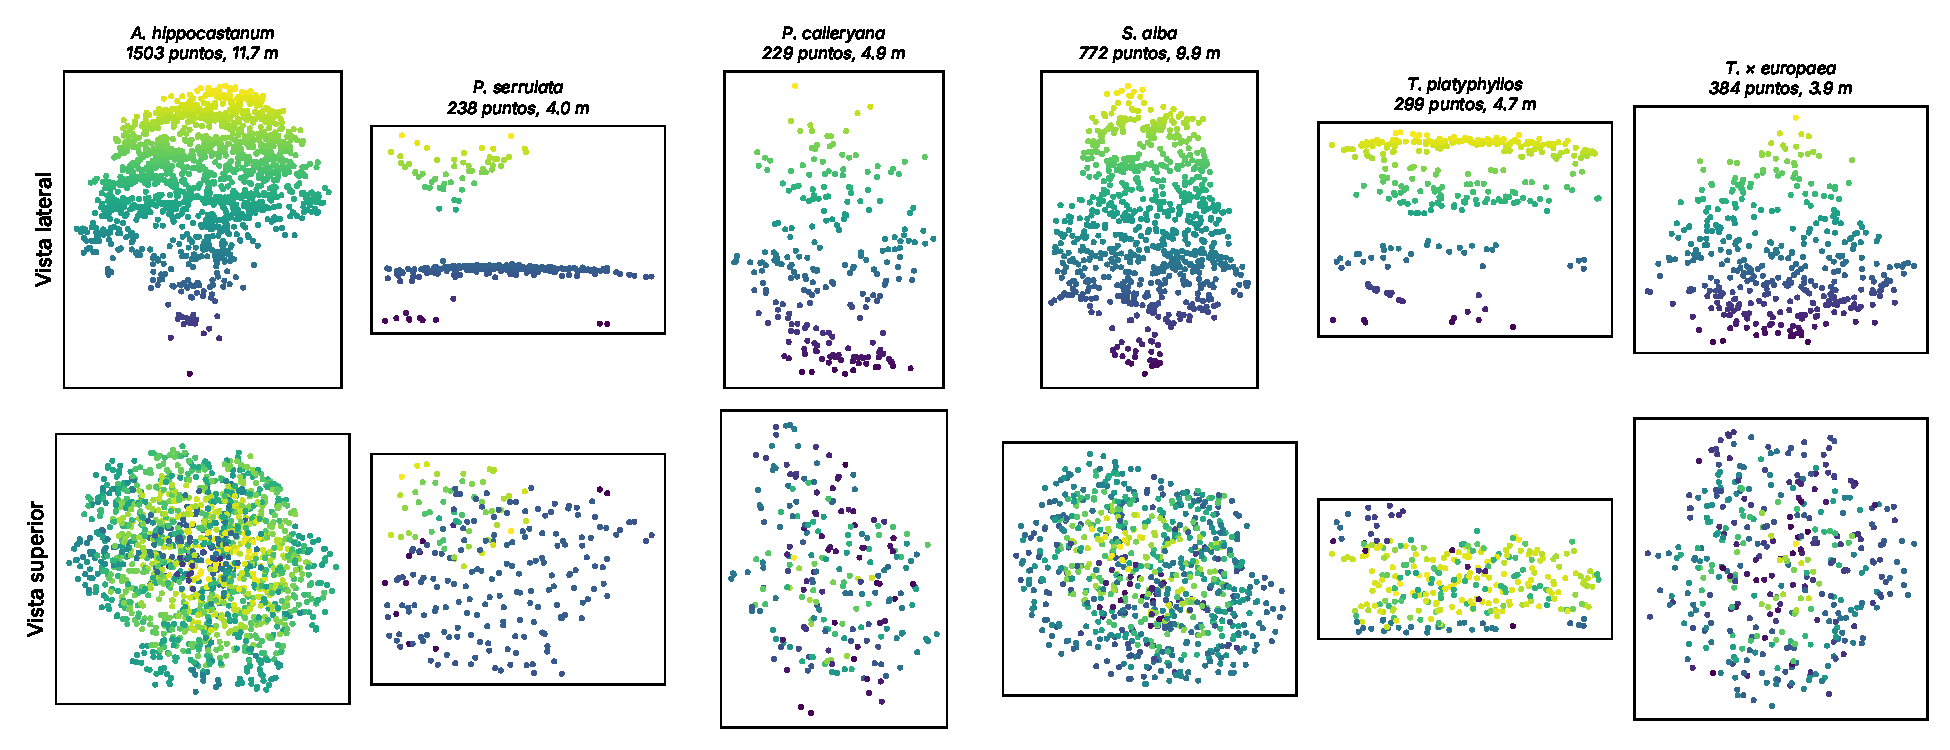
\includegraphics[width=0.72\textwidth]{figuras/ejemplos_dataset.pdf}
\caption{Un árbol de cada especie de UrbanTree3D en vista lateral y superior, con los puntos coloreados según su altura.}
\label{fig:ejemplos}
\end{figure}

\subsection{Preprocesamiento y aumento de datos}

Las nubes vienen filtradas y con la altura normalizada por los autores del dataset \cite{hamdani2026urbantree3d}. Para las redes, cada árbol se centra en su centroide y se escala a la esfera unitaria, de modo que la red recibe la forma y no el tamaño, y se muestrean $n$ puntos por árbol, con reemplazo cuando el árbol tiene menos. En entrenamiento la muestra cambia en cada época, mientras que en validación y prueba se fija con una semilla constante para que todos los modelos vean los mismos puntos.

Durante el entrenamiento cada árbol se rota al azar alrededor del eje vertical, se escala por eje con un factor entre 0.85 y 1.15, recibe ruido gaussiano de desviación 0.01 y pierde hasta 20\,\% de sus puntos. En la variante con atributos se agregan tres canales por punto, que son el logaritmo de la intensidad estandarizado con la media y la desviación del conjunto de entrenamiento, la razón entre el número de retorno y el total de retornos, y el total de retornos dividido entre ocho.

\subsection{Arquitecturas}

Las tres redes se implementaron en PyTorch, se muestran en la Figura~\ref{fig:arq} y comparten una cabeza de clasificación con capas de 512 y 256 unidades, normalización por lote y \textit{dropout} de 0.4.

\begin{figure}[!htbp]
\centering
\resizebox{0.8\textwidth}{!}{%
\begin{tikzpicture}[
  font=\footnotesize,
  caja/.style={draw, rounded corners=2pt, minimum height=0.95cm, minimum width=1.9cm, align=center, fill=blue!7},
  glob/.style={draw, rounded corners=2pt, minimum height=0.95cm, minimum width=1.9cm, align=center, fill=orange!15},
  sal/.style={draw, rounded corners=2pt, minimum height=0.95cm, minimum width=1.9cm, align=center, fill=green!12},
  flecha/.style={-{Stealth[length=2mm]}, thick}
]
\node[font=\bfseries, anchor=west] at (-1,2.6) {PointNet};
\node[caja] (a0) at (0,1.6) {Entrada\\$n\times d$};
\node[caja, right=0.4cm of a0] (a1) {MLP\\64, 128, 1024};
\node[glob, right=0.4cm of a1] (a2) {Máximo\\global};
\node[caja, right=0.4cm of a2] (a3) {FC\\512, 256};
\node[sal, right=0.4cm of a3] (a4) {Logits\\6};
\foreach \i/\j in {a0/a1,a1/a2,a2/a3,a3/a4} \draw[flecha] (\i) -- (\j);

\node[font=\bfseries, anchor=west] at (-1,0.45) {PointNet++};
\node[caja] (b0) at (0,-0.55) {Entrada\\$n\times d$};
\node[caja, right=0.4cm of b0] (b1) {SA1\\256 centros\\$r=0.2$, 32 vec.};
\node[caja, right=0.4cm of b1] (b2) {SA2\\64 centros\\$r=0.4$, 32 vec.};
\node[glob, right=0.4cm of b2] (b3) {MLP 256, 512,\\1024 y máximo};
\node[caja, right=0.4cm of b3] (b4) {FC\\512, 256};
\node[sal, right=0.4cm of b4] (b5) {Logits\\6};
\foreach \i/\j in {b0/b1,b1/b2,b2/b3,b3/b4,b4/b5} \draw[flecha] (\i) -- (\j);

\node[font=\bfseries, anchor=west] at (-1,-1.7) {DGCNN};
\node[caja] (c0) at (0,-2.7) {Entrada\\$n\times d$};
\node[caja, right=0.4cm of c0] (c1) {EdgeConv\\64, $k=16$};
\node[caja, right=0.4cm of c1] (c2) {EdgeConv\\64, $k=16$};
\node[caja, right=0.4cm of c2] (c3) {EdgeConv\\128, $k=16$};
\node[glob, right=0.4cm of c3] (c4) {Conv 1024,\\máximo y media};
\node[caja, right=0.4cm of c4] (c5) {FC\\512, 256};
\node[sal, right=0.4cm of c5] (c6) {Logits\\6};
\foreach \i/\j in {c0/c1,c1/c2,c2/c3,c3/c4,c4/c5,c5/c6} \draw[flecha] (\i) -- (\j);
\end{tikzpicture}}
\caption{Arquitecturas comparadas. $n$ es el número de puntos y $d$ los canales por punto, 3 con solo coordenadas y 6 con atributos. SA es una capa de abstracción de conjuntos, FC una capa totalmente conectada y $r$ el radio de agrupamiento.}
\label{fig:arq}
\end{figure}

\textbf{PointNet} transforma cada punto con un perceptrón compartido de 64, 128 y 1\,024 canales, obtiene un vector global con un máximo sobre los puntos y tiene 0.80 millones de parámetros. \textbf{PointNet++} usa dos capas de abstracción de conjuntos, y en cada una elige centros con muestreo del punto más lejano y agrupa hasta 32 vecinos con una consulta por radio, como en el artículo original \cite{qi2017pointnetpp}. Con nubes sobremuestreadas los 32 vecinos más cercanos serían copias del mismo punto, y por eso se usó la consulta por radio. Esta red tiene 1.46 millones de parámetros. \textbf{DGCNN} aplica tres capas EdgeConv sobre un grafo de 16 vecinos recalculado en cada capa, concatena sus salidas, las proyecta a 1\,024 canales, combina el máximo y la media globales y tiene 1.47 millones de parámetros.

\subsection{Baseline clásico}

El baseline es un bosque aleatorio \cite{breiman2001rf} de 500 árboles con pesos de clase balanceados, que siempre recibe la intensidad y los retornos del LiDAR. La variante sin escala usa 27 descriptores independientes del tamaño, entre ellos percentiles de altura normalizada, un histograma vertical de diez cajas, los valores propios normalizados de la covarianza, estadísticos del radio de copa y la media y la desviación de la intensidad y de los retornos. La variante con escala agrega la altura, el ancho de copa, su relación y el logaritmo del número de puntos, para un total de 31 descriptores.

\subsection{Entrenamiento}

Las redes se entrenan con entropía cruzada ponderada, donde el peso de la especie $c$ es la raíz cuadrada de la razón entre el promedio de ejemplos por clase y los ejemplos de esa clase.
\begin{equation}
\mathcal{L}(\theta) = -\frac{1}{B}\sum_{b=1}^{B} w_{y_b}\,\log \hat{p}_\theta\!\left(y_b \mid P_b\right), \qquad w_c = \sqrt{\frac{n}{C\,n_c}},
\label{eq:loss}
\end{equation}
donde $B$ es el tamaño del lote, $n$ el total de árboles de entrenamiento y $n_c$ los de la especie $c$. Se usa Adam \cite{kingma2015adam} con tasa inicial de $10^{-3}$, decaimiento de pesos de $10^{-4}$, un programa coseno de 100 épocas y lotes de 16 árboles, y las 100 épocas se eligieron para acercarse a las 105 del descriptor del dataset. En cada época se mide el F1 macro de validación y se conserva el mejor modelo, y como con 22 árboles de validación ese F1 llega a 1.0 en varias épocas, los empates se resuelven con la exactitud y luego con la menor pérdida de validación.

\subsection{Protocolo experimental}

Se hicieron cuatro experimentos.
\begin{enumerate}
\item \textbf{Partición oficial.} Se entrenan los cinco métodos con 1\,024 puntos, usando solo coordenadas en las redes y las semillas 0, 5 y 95 del descriptor del dataset.
\item \textbf{Número de puntos.} Se entrenan PointNet y PointNet++ con 1\,024, 2\,048, 4\,096 y 8\,192 puntos en la partición oficial.
\item \textbf{Atributos del sensor.} Las tres redes reciben las coordenadas, la intensidad y los retornos en la partición oficial.
\item \textbf{Validación cruzada repetida.} Los 152 árboles se dividen en cinco pliegues estratificados por especie, y en cada pliegue uno es la prueba y del resto se separa un 15\,\% estratificado como validación. El proceso se repite tres veces con particiones distintas, lo que da 15 entrenamientos por método y deja cada árbol tres veces en prueba, y se evalúan los dos bosques aleatorios y las tres redes con y sin atributos.
\end{enumerate}

Las métricas se calculan con la matriz de confusión $M$, donde $M_{ij}$ cuenta los árboles de la especie $i$ predichos como $j$.
\begin{equation}
\mathrm{Exactitud} = \frac{\sum_c M_{cc}}{\sum_{i,j} M_{ij}}, \quad F_{1,c} = \frac{2\,M_{cc}}{\sum_j M_{cj} + \sum_i M_{ic}}, \quad F_{1}^{\text{macro}} = \frac{1}{C}\sum_{c=1}^{C} F_{1,c}.
\label{eq:metrics}
\end{equation}
La exactitud balanceada es el promedio de la exhaustividad por clase, y como las clases están desbalanceadas el F1 macro es la métrica principal. En los experimentos 1 a 3 se reporta la media y la desviación estándar de las tres semillas, mientras que en el experimento 4 las predicciones de los cinco pliegues de cada repetición se juntan para calcular las métricas sobre los 152 árboles y se reporta la media y la desviación de las tres repeticiones. El intervalo de confianza de 95\,\% se obtiene con 2\,000 remuestreos \textit{bootstrap} de los árboles.

\subsection{Pruebas estadísticas}

Cada par de métodos del experimento 4 se compara con dos pruebas, y la primera es la prueba t corregida de Nadeau y Bengio, que usa el F1 de los $J=15$ pliegues. Como los conjuntos de entrenamiento se solapan entre pliegues, la prueba t normal subestima la varianza, y la corrección la multiplica por un factor que depende de la razón entre los tamaños de prueba y de entrenamiento \cite{nadeau2003inference}.
\begin{equation}
t = \frac{\bar{d}}{\sqrt{\left(\frac{1}{J} + \frac{n_{\text{prueba}}}{n_{\text{entren}}}\right)\hat{\sigma}_d^{2}}},
\label{eq:nb}
\end{equation}
donde $\bar{d}$ y $\hat{\sigma}_d^2$ son la media y la varianza de las diferencias de F1 entre los dos métodos, y la razón entre los tamaños de prueba y de entrenamiento es 0.25. La prueba exacta de McNemar compara los aciertos sobre los mismos 152 árboles en cada repetición, usando solo los casos en que un método acierta y el otro falla \cite{dietterich1998tests}. Como hay 28 pares, los valores p de cada prueba se ajustan con el método de Holm \cite{holm1979simple}, y una diferencia se considera significativa si el valor ajustado es menor que 0.05.

\subsection{Implementación y reproducibilidad}

Todo el experimento está en un notebook que descarga los datos desde Zenodo, entrena los modelos y genera las tablas y figuras. Se ejecutó en Google Colab con una GPU NVIDIA T4, PyTorch 2.14.1 y Python 3.13, y todas las cifras de este documento salen del archivo de resumen que produce.

%% =====================================================================
\section{Resultados}
\label{sec:resultados}

\subsection{Partición oficial}

La Tabla~\ref{tab:e1} resume el experimento 1, en el que DGCNN obtuvo el mejor F1 macro de prueba con 0.964, seguido por PointNet con 0.936, el bosque aleatorio sin escala con 0.906, el bosque aleatorio con escala con 0.864 y PointNet++ con 0.815. Con 26 árboles de prueba un error equivale a 3.8 puntos de exactitud, y DGCNN falló un árbol y PointNet dos en cada semilla. PointNet++ fue el más inestable, con exactitudes entre 0.769 y 0.885 según la semilla. El F1 de validación de PointNet y DGCNN fue de 0.986, lo que muestra que 22 árboles de validación no bastan para distinguir entre modelos.

\begin{table}[!htbp]
\centering
\footnotesize
\resizebox{\textwidth}{!}{%
\begin{tabular}{lccccc}
\toprule
Método & Exactitud prueba & F1 macro prueba & Exact. balanceada prueba & F1 macro validación & Parám. (M) \\
\midrule
RF con escala & 0.872 $\pm$ 0.022 & 0.864 $\pm$ 0.023 & 0.872 $\pm$ 0.024 & 0.821 $\pm$ 0.014 & -- \\
RF sin escala & 0.910 $\pm$ 0.022 & 0.906 $\pm$ 0.016 & 0.922 $\pm$ 0.010 & 0.813 $\pm$ 0.033 & -- \\
PointNet & 0.923 $\pm$ 0.000 & 0.936 $\pm$ 0.000 & 0.942 $\pm$ 0.000 & 0.986 $\pm$ 0.025 & 0.80 \\
PointNet++ & 0.833 $\pm$ 0.059 & 0.815 $\pm$ 0.052 & 0.851 $\pm$ 0.063 & 0.835 $\pm$ 0.051 & 1.46 \\
DGCNN & 0.962 $\pm$ 0.000 & 0.964 $\pm$ 0.005 & 0.983 $\pm$ 0.000 & 0.986 $\pm$ 0.025 & 1.47 \\
\bottomrule

\end{tabular}}
\caption{Experimento 1, partición oficial con 1\,024 puntos. Media y desviación de tres semillas sobre 26 árboles de prueba y 22 de validación.}
\label{tab:e1}
\end{table}


\subsection{Número de puntos por árbol}

La Tabla~\ref{tab:e2} muestra el experimento 2. PointNet se mantuvo entre 0.910 y 0.943 de F1 con cualquier número de puntos, mientras que PointNet++ mejoró de 0.815 con 1\,024 puntos a 0.842 con 4\,096 y cayó a 0.743 con 8\,192, con una desviación de 0.119 entre semillas. El costo también creció con los puntos, porque el tiempo medio de entrenamiento de PointNet pasó de 17 a 77 segundos y el de PointNet++ de 58 a 138 segundos.

\begin{table}[!htbp]
\centering
\footnotesize
\resizebox{\textwidth}{!}{%
\begin{tabular}{lccccc}
\toprule
Red & Puntos & Exactitud prueba & F1 macro prueba & Exactitud validación & Tiempo (s) \\
\midrule
PointNet & 1\,024 & 0.923 $\pm$ 0.000 & 0.936 $\pm$ 0.000 & 0.985 $\pm$ 0.026 & 17 \\
PointNet & 2\,048 & 0.923 $\pm$ 0.000 & 0.920 $\pm$ 0.028 & 0.985 $\pm$ 0.026 & 21 \\
PointNet & 4\,096 & 0.923 $\pm$ 0.038 & 0.910 $\pm$ 0.051 & 1.000 $\pm$ 0.000 & 38 \\
PointNet & 8\,192 & 0.936 $\pm$ 0.022 & 0.943 $\pm$ 0.022 & 1.000 $\pm$ 0.000 & 77 \\
\midrule
PointNet++ & 1\,024 & 0.833 $\pm$ 0.059 & 0.815 $\pm$ 0.052 & 0.879 $\pm$ 0.052 & 58 \\
PointNet++ & 2\,048 & 0.859 $\pm$ 0.044 & 0.822 $\pm$ 0.085 & 0.939 $\pm$ 0.052 & 62 \\
PointNet++ & 4\,096 & 0.872 $\pm$ 0.022 & 0.842 $\pm$ 0.017 & 0.909 $\pm$ 0.000 & 74 \\
PointNet++ & 8\,192 & 0.769 $\pm$ 0.102 & 0.743 $\pm$ 0.119 & 0.848 $\pm$ 0.026 & 138 \\
\bottomrule

\end{tabular}}
\caption{Experimento 2, número de puntos por árbol en la partición oficial. Media y desviación de tres semillas. El tiempo es el promedio por entrenamiento en la GPU T4.}
\label{tab:e2}
\end{table}

\subsection{Atributos del sensor}

Con intensidad y retornos en la partición oficial, PointNet clasificó bien los 26 árboles de prueba en las tres semillas, con exactitud y F1 de 1.000. PointNet++ subió de 0.833 a 0.974 de exactitud y de 0.815 a 0.972 de F1, y DGCNN pasó de 0.962 a 0.974 de exactitud y de 0.964 a 0.969 de F1.

\subsection{Evolución del entrenamiento}

La Figura~\ref{fig:curvas} muestra el entrenamiento de las tres redes con atributos y la semilla 0, con la pérdida de entrenamiento y de validación arriba y las métricas de validación con las que se elige la época abajo. La pérdida de entrenamiento se promedia sobre los lotes aumentados, con \textit{dropout} y pesos por clase, y la de validación se mide sin aumentos ni pesos, así que no son del todo equivalentes. El F1 con los datos de entrenamiento no se registró en los experimentos.

En las tres redes la pérdida de entrenamiento baja de cerca de 1.5 a unos 0.02, mientras que la de validación arranca entre 1.8 y 2.8, oscila durante las primeras 50 épocas y se estabiliza cuando baja la tasa de aprendizaje. El F1 de validación llegó a 1.0 por primera vez en la época 16 con PointNet, en la 24 con PointNet++ y en la 22 con DGCNN. Al final las dos pérdidas quedan parecidas y no se ve un sobreajuste marcado, aunque con 22 árboles de validación las métricas se saturan pronto.

\begin{figure}[!htbp]
\centering
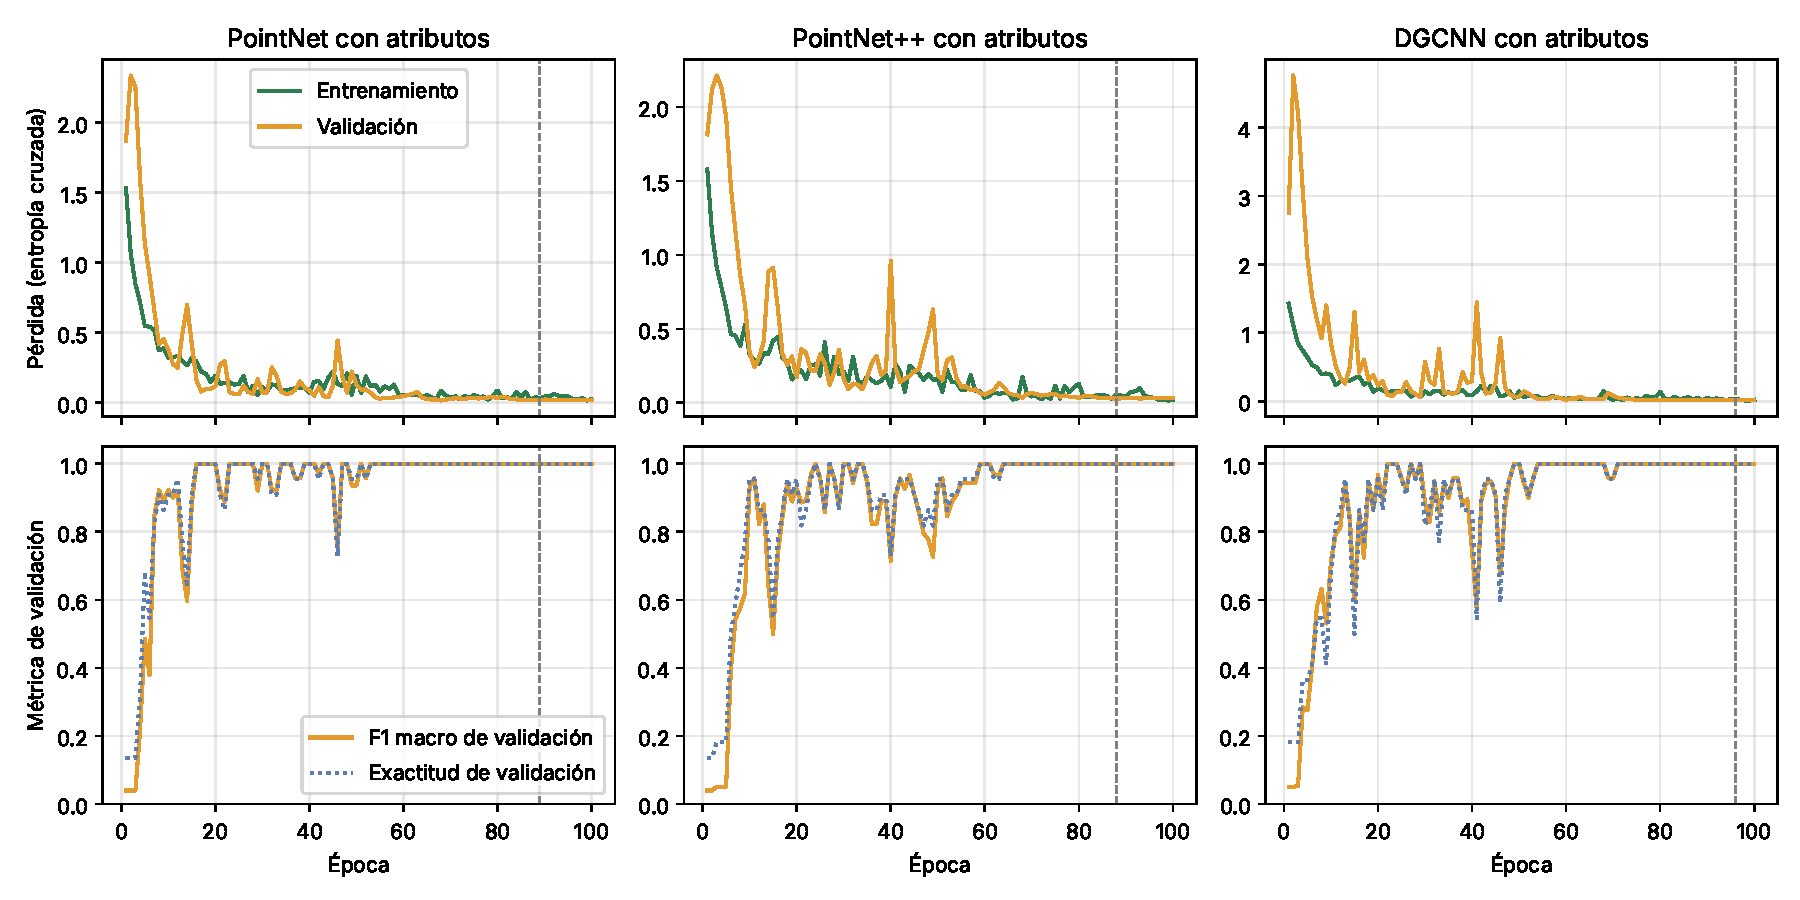
\includegraphics[width=0.78\textwidth]{figuras/curvas_entr_val.pdf}
\caption{Pérdida de entrenamiento y de validación (arriba) y métricas de validación (abajo) por época, para las tres redes con atributos y la semilla 0. La línea punteada vertical marca la época elegida.}
\label{fig:curvas}
\end{figure}

\subsection{Ejemplos de predicción}

La Figura~\ref{fig:pred} toma un árbol de prueba por especie de la partición oficial y compara su especie real con la que predijo cada red con atributos y la semilla 0. Cuando alguna red falla en una especie se muestra ese árbol. PointNet acertó los 26 árboles de prueba y PointNet++ y DGCNN fallaron uno cada una. DGCNN confundió el árbol 13902, un \textit{A. hippocastanum}, con un \textit{S. alba}, y PointNet++ confundió el árbol 13623, un \textit{P. calleryana}, con un \textit{T. platyphyllos}. En los dos casos las otras redes acertaron, y la tabla completa de los 26 árboles está en el notebook.

\begin{figure}[!htbp]
\centering
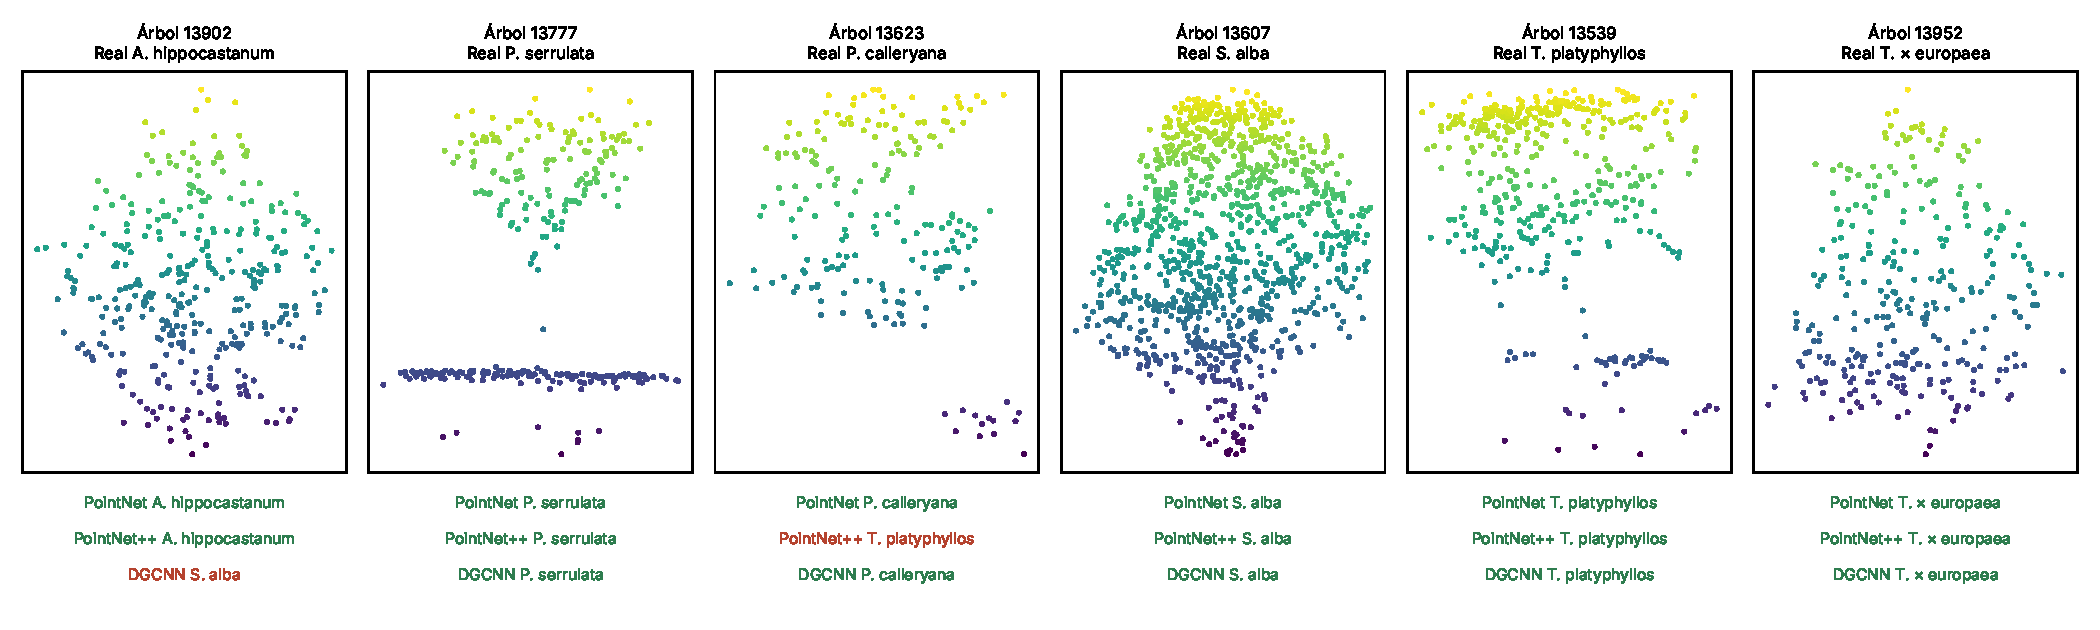
\includegraphics[width=0.85\textwidth]{figuras/predicciones.pdf}
\caption{Vista lateral de un árbol de prueba por especie con su especie real y la predicha por cada red con atributos (semilla 0). En verde las predicciones correctas y en rojo los errores.}
\label{fig:pred}
\end{figure}

\subsection{Validación cruzada repetida}

La Tabla~\ref{tab:e4} y la Figura~\ref{fig:cv} presentan el experimento 4, que evalúa los 152 árboles tres veces y en el que las cifras bajan frente a la partición oficial en todos los métodos. PointNet con atributos obtuvo el mejor resultado, con 0.928 de exactitud y 0.914 de F1 macro, seguido de cerca por DGCNN con atributos, con 0.923 y 0.910. PointNet++ con atributos y el bosque aleatorio con escala quedaron cerca de 0.85 de F1, los demás métodos entre 0.830 y 0.841 y PointNet++ sin atributos último, con 0.723.

\begin{table}[!htbp]
\centering
\footnotesize
\resizebox{\textwidth}{!}{%
\begin{tabular}{lccccc}
\toprule
Método & Exactitud & IC 95\,\% exactitud & F1 macro & IC 95\,\% F1 & Exact. balanceada \\
\midrule
RF con escala & 0.877 $\pm$ 0.017 & [0.827, 0.921] & 0.853 $\pm$ 0.014 & [0.784, 0.906] & 0.844 $\pm$ 0.015 \\
RF sin escala & 0.846 $\pm$ 0.014 & [0.792, 0.895] & 0.830 $\pm$ 0.017 & [0.761, 0.883] & 0.815 $\pm$ 0.022 \\
PointNet & 0.860 $\pm$ 0.017 & [0.816, 0.901] & 0.833 $\pm$ 0.021 & [0.776, 0.877] & 0.847 $\pm$ 0.012 \\
PointNet++ & 0.772 $\pm$ 0.039 & [0.715, 0.820] & 0.723 $\pm$ 0.045 & [0.653, 0.779] & 0.746 $\pm$ 0.038 \\
DGCNN & 0.866 $\pm$ 0.034 & [0.822, 0.904] & 0.841 $\pm$ 0.033 & [0.788, 0.882] & 0.864 $\pm$ 0.035 \\
PointNet + atributos & 0.928 $\pm$ 0.024 & [0.893, 0.956] & 0.914 $\pm$ 0.030 & [0.868, 0.948] & 0.918 $\pm$ 0.025 \\
PointNet++ + atributos & 0.875 $\pm$ 0.017 & [0.833, 0.912] & 0.858 $\pm$ 0.024 & [0.804, 0.901] & 0.864 $\pm$ 0.039 \\
DGCNN + atributos & 0.923 $\pm$ 0.019 & [0.890, 0.952] & 0.910 $\pm$ 0.023 & [0.865, 0.943] & 0.920 $\pm$ 0.026 \\
\bottomrule

\end{tabular}}
\caption{Experimento 4, validación cruzada estratificada de cinco pliegues repetida tres veces. Media y desviación entre repeticiones e intervalo de confianza \textit{bootstrap} de 95\,\%.}
\label{tab:e4}
\end{table}

\begin{figure}[!ht]
\centering
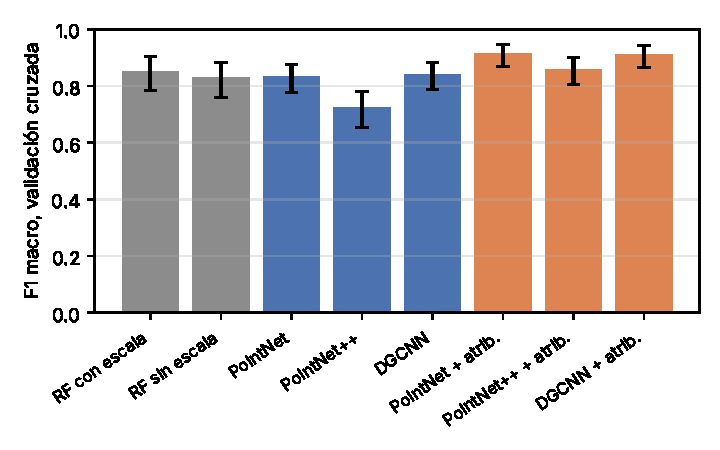
\includegraphics[width=0.46\textwidth]{figuras/cv_f1.pdf}
\caption{F1 macro en validación cruzada con su intervalo de confianza de 95\,\%. Gris indica el bosque aleatorio, azul las redes con solo coordenadas y naranja las redes con atributos.}
\label{fig:cv}
\end{figure}

La Tabla~\ref{tab:clases} muestra el F1 por especie. \textit{Pyrus calleryana} fue la más difícil para todos los métodos, con valores entre 0.56 y 0.83, y los atributos mejoraron sobre todo esa especie y \textit{Tilia $\times$ europaea}, que en PointNet++ pasó de 0.62 a 0.92.

\begin{table}[!ht]
\centering
\footnotesize
\resizebox{\textwidth}{!}{%
\begin{tabular}{lcccccc}
\toprule
Método & \textit{A. hippocastanum} & \textit{P. serrulata} & \textit{P. calleryana} & \textit{S. alba} & \textit{T. platyphyllos} & \textit{T. $\times$ europaea} \\
\midrule
RF con escala & 0.92 & 0.92 & 0.76 & 0.87 & 0.89 & 0.74 \\
RF sin escala & 0.87 & 0.92 & 0.75 & 0.84 & 0.89 & 0.71 \\
PointNet & 0.91 & 0.86 & 0.62 & 0.81 & 0.91 & 0.89 \\
PointNet++ & 0.86 & 0.67 & 0.56 & 0.80 & 0.83 & 0.62 \\
DGCNN & 0.90 & 0.83 & 0.65 & 0.87 & 0.92 & 0.87 \\
PointNet + atributos & 0.95 & 0.92 & 0.82 & 0.92 & 0.92 & 0.95 \\
PointNet++ + atributos & 0.90 & 0.88 & 0.73 & 0.83 & 0.89 & 0.92 \\
DGCNN + atributos & 0.95 & 0.93 & 0.83 & 0.90 & 0.93 & 0.91 \\
\bottomrule

\end{tabular}}
\caption{F1 por especie en validación cruzada, promedio de las tres repeticiones.}
\label{tab:clases}
\end{table}

La Figura~\ref{fig:confusion} compara las matrices de confusión de PointNet con atributos y del bosque aleatorio sin escala, sumadas sobre las tres repeticiones. PointNet con atributos acertó 423 de 456 casos y su error más frecuente fue confundir \textit{Pyrus calleryana} con \textit{Tilia platyphyllos}, mientras que el bosque aleatorio sin escala acertó 386 y se confundió sobre todo entre \textit{Aesculus hippocastanum} y \textit{Tilia $\times$ europaea}, con 22 casos.

\begin{figure}[!ht]
\centering
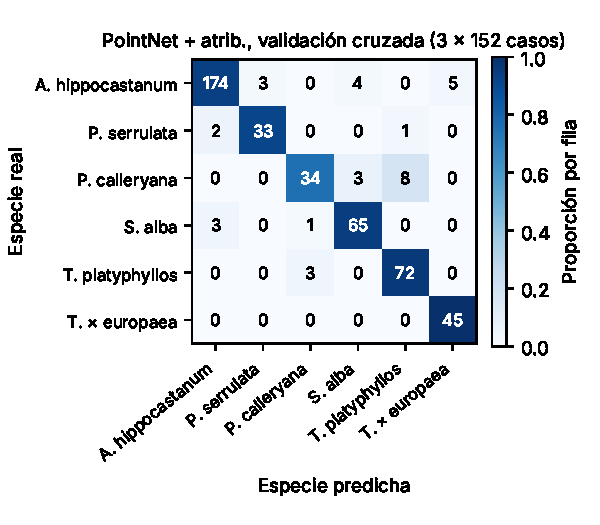
\includegraphics[width=0.36\textwidth]{figuras/confusion_cv.pdf}
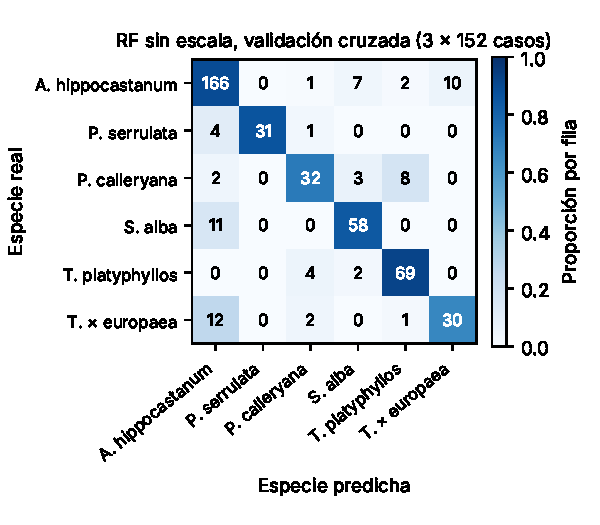
\includegraphics[width=0.36\textwidth]{figuras/confusion_cv_rf.pdf}
\caption{Matrices de confusión de PointNet con atributos y del bosque aleatorio sin escala en validación cruzada, con los conteos sumados de las tres repeticiones.}
\label{fig:confusion}
\end{figure}

\subsection{Comparación estadística}

La Tabla~\ref{tab:pares} resume las comparaciones más relevantes de los 28 pares, que están completas en el notebook. Con la prueba t corregida ninguna diferencia fue significativa después del ajuste de Holm, y el menor valor p sin ajustar fue 0.021, para PointNet++ frente a DGCNN con atributos. Con McNemar y Holm solo dos pares fueron significativos en las tres repeticiones, que son PointNet++ sin atributos frente a PointNet con atributos y frente a DGCNN con atributos.

\begin{table}[!ht]
\centering
\footnotesize
\resizebox{\textwidth}{!}{%
\begin{tabular}{llcccccc}
\toprule
Método A & Método B & Dif. F1 (A$-$B) & p t corregida & p Holm & Solo A / solo B & p Holm McNemar & Rep. signif. \\
\midrule
RF con escala & PointNet + atributos & -0.057 & 0.269 & 1.000 & 15 / 38 & 1.000 & 0 \\
RF sin escala & DGCNN + atributos & -0.088 & 0.086 & 1.000 & 14 / 49 & 1.000 & 0 \\
PointNet & PointNet + atributos & -0.079 & 0.094 & 1.000 & 14 / 45 & 1.000 & 1 \\
DGCNN & DGCNN + atributos & -0.066 & 0.257 & 1.000 & 11 / 37 & 1.000 & 1 \\
PointNet++ & PointNet++ + atributos & -0.143 & 0.096 & 1.000 & 29 / 76 & 1.000 & 2 \\
PointNet + atributos & DGCNN + atributos & -0.004 & 0.936 & 1.000 & 19 / 17 & 1.000 & 0 \\
PointNet++ & PointNet + atributos & -0.197 & 0.025 & 0.670 & 16 / 87 & 0.003 & 3 \\
PointNet++ & DGCNN + atributos & -0.201 & 0.021 & 0.596 & 18 / 87 & 0.020 & 3 \\
\bottomrule

\end{tabular}}
\caption{Comparaciones seleccionadas en validación cruzada. La diferencia de F1 es la media de los 15 pliegues. \textit{Solo A / solo B} cuenta los casos que acierta un solo método, sumados en las tres repeticiones. La p de McNemar es la mayor de las tres repeticiones después de Holm, y la última columna dice en cuántas repeticiones fue menor que 0.05.}
\label{tab:pares}
\end{table}

%% =====================================================================
\section{Discusión}
\label{sec:discusion}

\subsection{La partición oficial sobrestima el desempeño}

En la partición oficial DGCNN llegó a 0.964 de F1 y PointNet con atributos a 1.000, pero en validación cruzada las mismas configuraciones quedaron en 0.841 y 0.914. Las redes bajaron entre 0.09 y 0.12 mientras que el bosque aleatorio con escala solo bajó 0.012, así que los 26 árboles de prueba oficiales resultaron más fáciles que el promedio y un resultado perfecto en ellos no significa que el problema esté resuelto. Además PointNet con atributos fue de 0.679 a 1.000 de F1 según el pliegue, lo que coincide con la advertencia de Fassnacht et al. sobre los estudios que comparan algoritmos sin medir su incertidumbre \cite{fassnacht2016review}.

\subsection{Los atributos del sensor aportan más que la arquitectura}

En validación cruzada, agregar intensidad y retornos subió el F1 macro en 0.081 para PointNet, 0.069 para DGCNN y 0.135 para PointNet++, mientras que la diferencia entre PointNet y DGCNN fue de apenas 0.008 sin atributos y de 0.004 con ellos, así que la información del sensor pesó más que la elección de la red. Los retornos reflejan la porosidad de la copa y la intensidad depende de la reflectancia de las hojas. Briechle et al., Wang et al., Murray et al. y Vahrenhold et al. también mejoraron la clasificación al sumar información del sensor o descriptores a la nube \cite{briechle2020pointnetpp,wang2024rse,murray2025dualstream,vahrenhold2025mmtscnet}, y este trabajo encuentra el mismo efecto con LiDAR monoespectral.

Esto explica por qué el bosque aleatorio, que siempre recibió esos datos, fue tan competitivo en el experimento 1. Con la misma información las redes lo superaron por 0.06 de F1, sin que la ventaja fuera significativa, algo parecido a lo que Taher et al. observaron con LiDAR disperso \cite{taher2026msals}.

\subsection{Arquitectura y número de puntos}

PointNet, la red más simple, igualó a DGCNN y superó a PointNet++ en todos los experimentos, como en Hamdani et al. con otro dataset urbano \cite{hamdani2026classification}, y en línea con Qian et al., para quienes el entrenamiento pesa tanto como la arquitectura \cite{qian2022pointnext}.

El descriptor del dataset usó PointNet++ con 8\,192 puntos y reportó entre 0.94 y 0.96 de exactitud de validación \cite{hamdani2026urbantree3d}. Aquí PointNet++ alcanzó 0.939 con 2\,048 puntos pero bajó a 0.848 con 8\,192, porque con una mediana de 429 puntos por árbol casi toda esa muestra son repeticiones. PointNet no depende de vecindarios locales y no se vio afectado, y el rango útil coincide con el de Zhang et al. \cite{zhang2025uav}.

\subsection{Comparación con trabajos similares}

La Tabla~\ref{tab:literatura} ubica estos resultados frente a trabajos cercanos, aunque las cifras no son directamente comparables porque cambian el sensor, las especies y el protocolo.

\begin{table}[!htbp]
\centering
\scriptsize
\renewcommand{\arraystretch}{1.1}
\begin{tabular}{>{\raggedright\arraybackslash}p{2.1cm} >{\raggedright\arraybackslash}p{3.3cm} >{\raggedright\arraybackslash}p{1.0cm} >{\raggedright\arraybackslash}p{2.4cm} >{\raggedright\arraybackslash}p{2.8cm}}
\toprule
Trabajo & Datos & Especies & Mejor método & Resultado \\
\midrule
Hamdani et al. \cite{hamdani2026urbantree3d} & UrbanTree3D, LiDAR aéreo urbano & 6 & PointNet++, 8\,192 puntos & Exactitud de validación de 0.94 a 0.96 \\
Hamdani et al. \cite{hamdani2026classification} & LiDAR multiespectral urbano & -- & PointNet & Exactitud de prueba de 0.821 \\
Briechle et al. \cite{briechle2020pointnetpp} & LiDAR de UAV y multiespectral & 3 + muertos & PointNet++ & Exactitud de 0.902, RF 0.853 \\
Taher et al. \cite{taher2026msals} & LiDAR aéreo multiespectral & -- & Point Transformer, RF con datos dispersos & Exactitud de 0.879, y 0.799 con datos dispersos \\
Murray et al. \cite{murray2025dualstream} & LiDAR aéreo boreal, 16\,269 árboles & 4 & Red de doble flujo & F1 ponderado de 0.70 \\
Puliti et al. \cite{puliti2025forspecies} & FOR-species20K, TLS, MLS y UAV & 33 & Modelos multivista & Exactitud promedio de 0.77 \\
Este trabajo & UrbanTree3D, validación cruzada repetida & 6 & PointNet con atributos & Exactitud de 0.928, F1 macro de 0.914 \\
\bottomrule
\end{tabular}
\caption{Resultados de trabajos similares. Un guion indica que el dato no se reporta en los resúmenes consultados.}
\label{tab:literatura}
\end{table}

El resultado es alto frente a FOR-species20K o al bosque boreal de Murray et al., pero aquí son seis especies urbanas bien separadas, y frente al descriptor de UrbanTree3D la diferencia principal es que aquí se mide en prueba con validación cruzada.

\subsection{Errores y limitaciones}

La confusión entre \textit{Aesculus hippocastanum} y \textit{Tilia $\times$ europaea}, que el descriptor del dataset también reporta \cite{hamdani2026urbantree3d}, se explica por copas de tamaño y densidad parecidos, y \textit{Pyrus calleryana} se confundió con \textit{Tilia platyphyllos} porque ambas tienen copas compactas y es una de las especies con menos árboles.

Las limitaciones son el tamaño del dataset, los puntos ajenos al árbol en algunas nubes y que todo viene de una sola ciudad y una sola campaña de vuelo, además de que solo se clasifica el árbol aislado.

%% =====================================================================
\section{Conclusiones y trabajo futuro}
\label{sec:conclusiones}

Este trabajo comparó PointNet, PointNet++ y DGCNN con un bosque aleatorio para clasificar seis especies de árboles urbanos en UrbanTree3D. La partición oficial resultó optimista, porque las redes que alcanzaron entre 0.96 y 1.00 de F1 en sus 26 árboles de prueba bajaron entre 0.06 y 0.12 en validación cruzada repetida, y con datasets tan pequeños conviene reportar ese tipo de validación con intervalos de confianza. Los atributos del LiDAR mejoraron las tres redes más que cualquier cambio de arquitectura, y PointNet con intensidad y retornos obtuvo el mejor resultado, con 0.928 de exactitud y 0.914 de F1 macro. La red más simple fue suficiente, porque PointNet igualó a DGCNN y superó a PointNet++, que además fue sensible al sobremuestreo. Con 152 árboles las pruebas corregidas solo confirmaron que PointNet++ sin atributos es inferior a las dos mejores redes con atributos, y la ventaja de las redes con atributos sobre el bosque aleatorio es consistente pero no significativa.

Como trabajo futuro se propone ampliar el dataset o preentrenar con FOR-species20K, probar arquitecturas como PointNeXt con el mismo protocolo, limpiar los puntos ajenos a cada árbol e integrar la segmentación y la clasificación en un solo flujo.

El notebook ejecutado y los resultados de cada entrenamiento están en \url{https://github.com/JDav19/arbolado-urbantree3d}, y el dataset está en Zenodo con DOI 10.5281/zenodo.19475932.

\renewcommand{\bibfont}{\footnotesize}
\setlength{\bibsep}{0pt}
\bibliographystyle{elsarticle-num}
\bibliography{referencias}

\end{document}
